\documentclass[border=4pt]{standalone}
% Preámbulo común de las figuras. Cada figura es un documento standalone
% que se compila a SVG con scripts/build_figures.sh
\usepackage[utf8]{inputenc}
\usepackage{amsmath}
\usepackage{tikz}
\usepackage[american, siunitx]{circuitikz}
\usetikzlibrary{arrows.meta,calc,decorations.pathmorphing,patterns}
\tikzset{
  >={Stealth[length=2.2mm]},
  eje/.style={->, thin},
  hilo/.style={thick},
}
% Paleta común: tonos medios legibles sobre fondo claro
\definecolor{azul}{RGB}{31,94,168}
\definecolor{rojo}{RGB}{192,57,43}
\definecolor{verde}{RGB}{39,128,73}
\definecolor{naranja}{RGB}{211,120,30}
\definecolor{morado}{RGB}{125,60,152}

\begin{document}
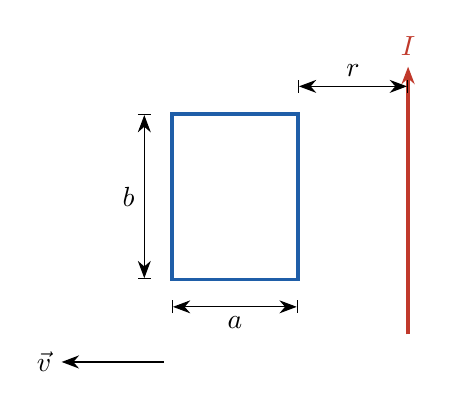
\begin{tikzpicture}[scale=1.0]
  \draw[very thick, rojo, ->] (4.0,-0.2) -- (4.0,3.2) node[above]{$I$};
  \draw[very thick, azul] (1.0,0.5) rectangle (2.6,2.6);
  \draw[|<->|] (2.6,2.95) -- node[above]{$r$} (4.0,2.95);
  \draw[|<->|] (1.0,0.15) -- node[below]{$a$} (2.6,0.15);
  \draw[|<->|] (0.65,0.5) -- node[left]{$b$} (0.65,2.6);
  \draw[->, thick] (0.9,-0.55) -- (-0.4,-0.55) node[left]{$\vec{v}$};
\end{tikzpicture}
\end{document}
